\begin{frame}
\frametitle{Понятие процесса}

Процесс - контейнер ресурсов ОС:
\begin{itemize}
  \item<2-> ресурсы в ОС привязаны к процессам
    \begin{itemize}
      \item память (свое адресное пространство у процессов)
      \item файловые дескрипторы
      \item другие ресурсы (сокеты, различные IPC и тд)
    \end{itemize}
  \item<3-> процессы изолированы друг от друга
    \begin{itemize}
      \item на сколько это позволяет аппаратное обеспечение (далее просто HW)
      \item некоторые процессы могут разделять общие ресурсы намеренно
    \end{itemize}
\end{itemize}

\end{frame}

\begin{frame}
\frametitle{Адресное пространство процесса}

Адресное пространство процесса (виртуальное адресное пространство, VA) - это набор адресов доступных процессу для работы (мы называем эти адреса виртуальными):

\begin{itemize}
  \item<2-> VA отображается на физическую память (далее PA)
    \begin{itemize}
      \item paging - произвольное отображение
      \item "один к одному", если HW не поддерживает трансляцию
    \end{itemize}
  \item<3-> VA может быть аппаратно защищено
    \begin{itemize}
      \item сегментирование - попытка обращения в чужой сегмент приводит к ошибке
      \item paging устраняет саму возможность обратиться к чужой памяти
    \end{itemize}
  \item<4-> VA может быть неоднородным - в нем могут быть дыры
\end{itemize}
\end{frame}

\begin{frame}
\frametitle{Адресное пространство процесса}

VA процесса - это ресурс, который нужно аллоцировать и освобождать:
\begin{itemize}
  \item<2-> ОС необходимо делить память между несколькими процессами - не нужно
выдавать процессу сразу много памяти, которая скорее всего не будет
использрована;
  \item<3-> разные части VA используются под разные нужды:
    \begin{itemize}
      \item они находятся в разных регионах VA (стек растет вниз, его логично положить наверх)
      \item могут иметь разные права/привилегии доступа (например, делать стек исполняемым - плохая затея с точки зрения безопасности)
    \end{itemize}
\end{itemize}
\end{frame}

\begin{frame}
\frametitle{Сегментация на примере x86}

Вся память разбивается на сегменты:
\begin{itemize}
  \item уровень привилегий доступа назначается каждому сегменту отдельно
  \item сегменты могут перекрываться, т. е. два сегмента с разными привилегиями могут описывать одну и ту же физическую память
\end{itemize}

\end{frame}

\begin{frame}
\frametitle{Сегментация на примере x86}

\begin{figure}
\centering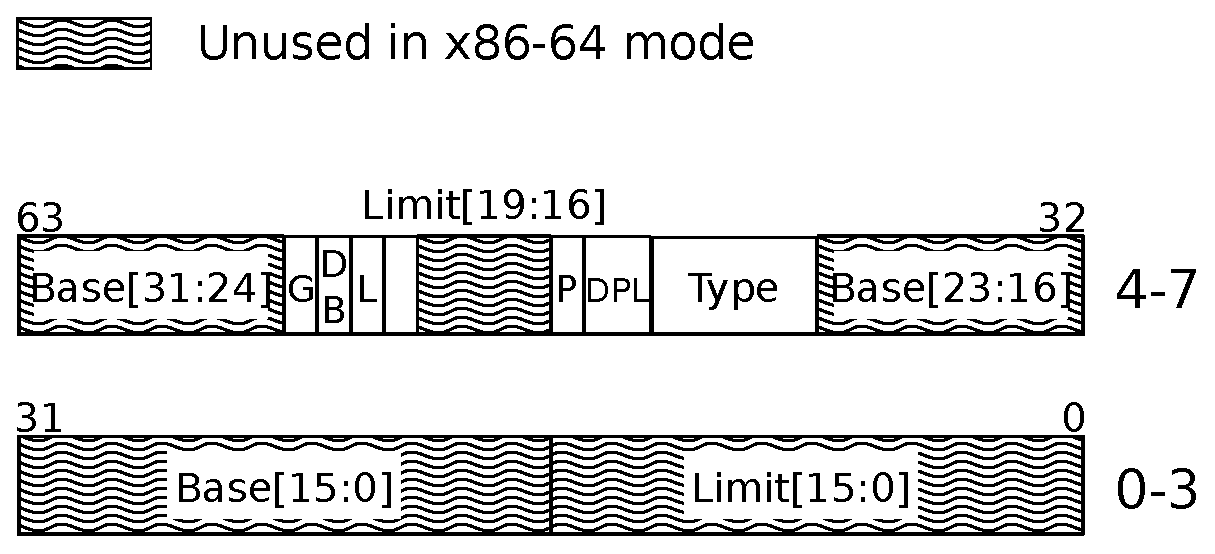
\includegraphics[width=.9\linewidth]{arch-segd}
\caption{x86 segment data/code descriptor format}
\end{figure}

\end{frame}

\begin{frame}
\frametitle{Сегментация на примере x86}

Дескрипторы сегментов хранятся в таблицах GDT и LDT:
\begin{itemize}
  \item GDT предполагается общей для всех процессов (не обязательно)
  \item LDT своя для каждого процесса (не обязательно)
  \item при обращении к памяти таблица и номер дескриптора в ней определяются используя селектор сегмента (16-битное значение в CS, SS, DS, ES, FS или GS)
\end{itemize}
\end{frame}

\begin{frame}
\frametitle{Сегментация на примере x86}

\begin{figure}
  \centering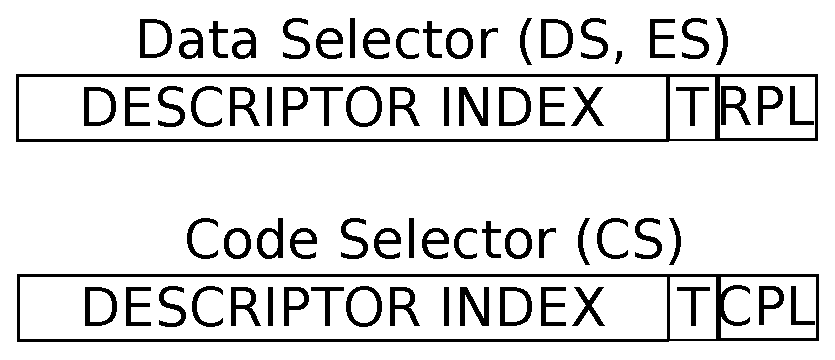
\includegraphics[width=.9\linewidth]{arch-segs}
  \caption{Code and Data Segment Selectors}
\end{figure}

\end{frame}

\begin{frame}
\frametitle{Сегментация на примере x86}

Проверка привилегий:
\begin{itemize}
  \item при записи селектора в сегментный регистр CPL (из CS) и RPL (то что мы записываем) должны быть меньше или равны DPL (в дескрипторе сегмента, на который мы ссылаемся);
  \item для селектора стека (SS) используются особые правила - RPL и DPL должны быть равны CPL.
\end{itemize}
\end{frame}
